\section{Introduction}
\frame{\sectionpage}

\begin{frame}{Motivation: Persistent Gender Pay Gap}

    \begin{figure}
        \centering
        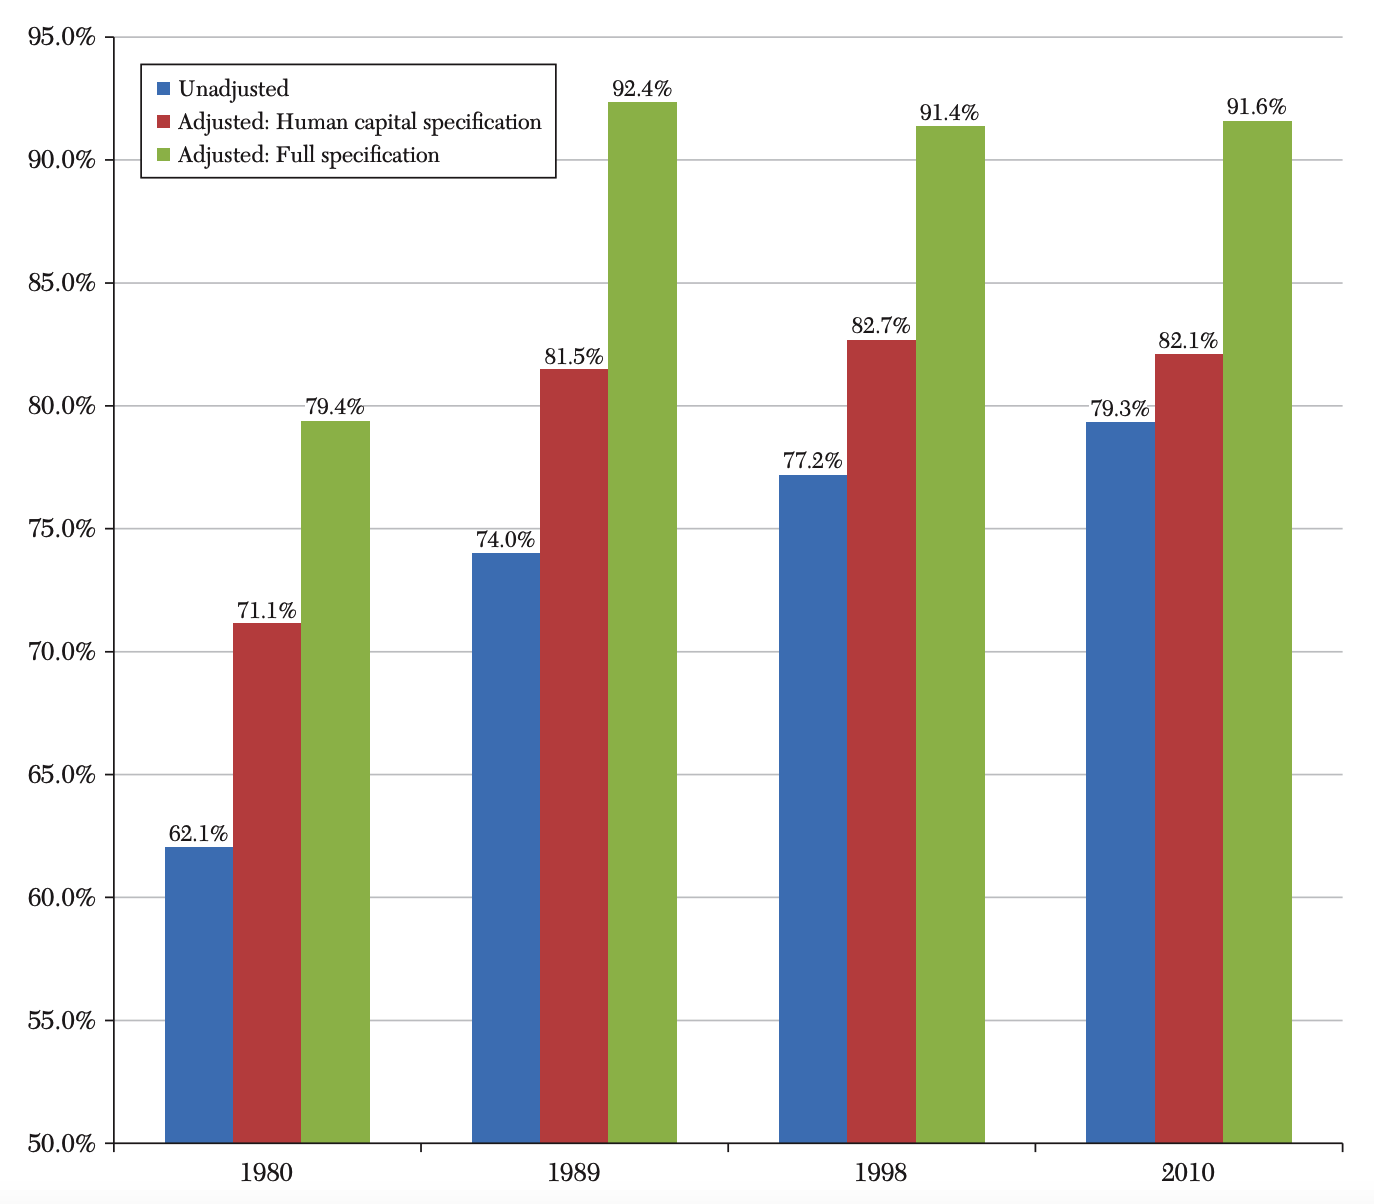
\includegraphics[height = 0.7 \textheight]{images/mot1.png}
        
        {\small \citet[Figure 2]{blau2017gender}}
    \end{figure}

\end{frame}

\begin{frame}{Motivation: Lower Salary Expectations of Women}

    \begin{figure}
        \centering
        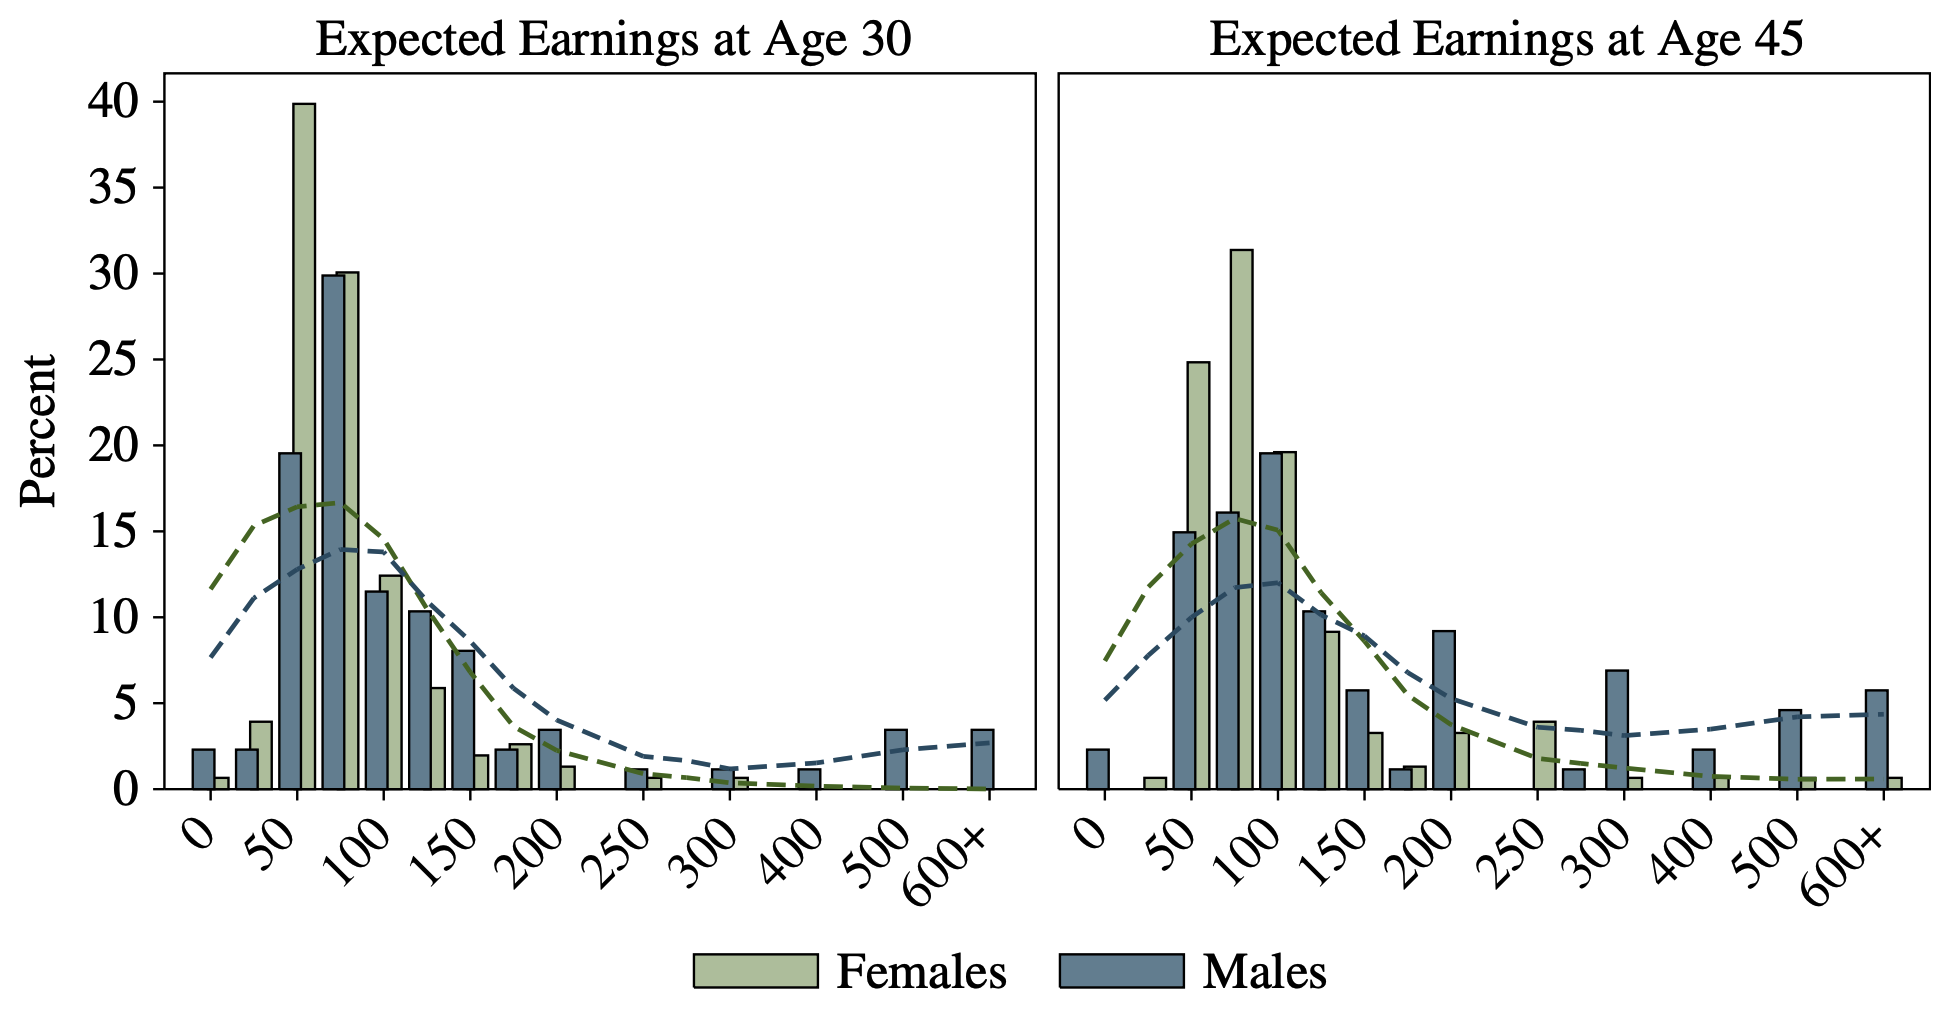
\includegraphics[height = 0.7 \textheight]{images/mot2.png}

        {\small \citet[Figure 1]{reuben2017preferences}}
    \end{figure}

\end{frame}

\begin{frame}{Motivation: Desired Salaries Are Asked During Hiring}
    \begin{table}[h!]
        \footnotesize
        \begin{center}
            \label{tab:BiasiSarsons}
            \begin{tabular}{lc}
            
                & Asked Desired Salary \\
               \hline
               Full sample & 40.08\% \\ \hline
               Male & 44\% \\
               Female & 36\% \\ \hline
               $<$ \$32K & 36\% \\
               \$32K-\$48K & 31\% \\
               \$48K-\$68K & 46\% \\
               $>$ \$68K & 55\% \\ \hline
               Architecture and engineering occupations & 91\% \\
               Computer and mathematical occupations & 46\% \\
               Unemployed & 31\% \\ \hline
            \end{tabular}
        \end{center}
    \end{table}
    \vspace*{-15pt}
    \begin{center}
        {\small \citet[Table A1-A3]{agan2020workers}}
    \end{center}
\end{frame}

\begin{frame}{Motivation: What's Missing?}
    \begin{block}{\textbf{So far}}
        \begin{itemize}
            \item \underline{\textit{salary expectation gaps}} likely contribute to persistent \underline{\textit{pay gaps}} 
            
            \hfill {\scriptsize \citet{babcock2003nice,leibbrandt2015women,biasi2022flexible}}
            \item \underline{\textit{desired salaries}} are indeed asked, and likely used, by recruiters
        \end{itemize}
    \end{block}

    \uncover<2->{
        \vspace*{10pt}
        \textbf{\underline{Empirical challenges}}
        \begin{itemize}
            \item<2-> desired salaries are rarely observed in real world recruitments
            \item<3-> wage data are often one sided \textcolor{frenchlilac!45!white}{\footnotesize (bargaining nature not captured)}
        \end{itemize}
    }
\end{frame}

\begin{frame}{Roadmap}
    \begin{center}
        A unique setting: Hired.com 
        
        {\footnotesize for \textcolor{frenchlilac!45!white}{\textit{\underline{high-wage engineering}}} jobs \hspace*{20pt} recording salary \textcolor{frenchlilac!45!white}{\textit{\underline{negotiation}}} components}
    \end{center}

    \uncover<2->{
        \begin{columns}[T]
            \uncover<3->{\begin{column}{0.3\textwidth}
                \begin{block}{\small \centering \textbf{Ask} Salary}
                \small \centering 
                by job seekers {\scriptsize \underline{\textit{with resume}}}
                \end{block}
                
                \uncover<6->{\footnotesize 
                \textcolor{frenchlilac!45!white}{\underline{$>$ \textbf{110,000}}} candidates
                \begin{itemize}
                    \footnotesize
                    \item<6-> raw gap: 6.8\%
                    \item<7-> \textit{net{\tiny -of-resume}} gap: \textcolor{frenchlilac!45!white}{\textbf{2.9\%}}
                \end{itemize}
                }
            \end{column}}
        
            \uncover<4->{\begin{column}{0.3\textwidth}
                \begin{block}{\small \centering \textbf{Bid} Salary}
                \small \centering
                by employers {\scriptsize \underline{\textit{pre-interview}}}
                \end{block}
                
                \uncover<6->{\footnotesize 
                    \textcolor{frenchlilac!45!white}{\underline{$>$ \textbf{460,000}}} bids
                    \begin{itemize}
                        \footnotesize
                        \item<6-> raw gap: 3.4\%{\tiny /4.9\%}
                        \item<7-> \textit{net} gap: \textcolor{frenchlilac!45!white}{\textbf{2.2\%{\tiny /1.8\%}}}
                    \end{itemize}
                    }

            \end{column}}

            \uncover<5->{\begin{column}{0.3\textwidth}
                \begin{block}{\small \centering \textbf{Final} Salary}
                \small \centering
                wage {\scriptsize \underline{\textit{post-negotiation}}} 
                \end{block}

                \uncover<6->{\footnotesize 
                    \textcolor{frenchlilac!45!white}{\underline{\textbf{7,582}}} hirings
                    \begin{itemize}
                        \footnotesize
                        \item<6-> raw gap: 4.9\%
                        \item<7-> \textit{net} gap: \textcolor{frenchlilac!45!white}{\textbf{1.4\%}}
                    \end{itemize}
                    }
                
            \end{column}}
        \end{columns}
    }

    \uncover<8>{
    \vspace*{20pt}
    \small    An \textcolor{frenchlilac!45!white}{\textit{\underline{information}}} treatment: providing median \textcolor{frenchlilac!45!white}{\textbf{\underline{bid}}} salary for similar candidates
    \vspace*{5pt}
}
    
\end{frame}

\begin{frame}{Contribution to the Literature}
    \begin{itemize}
        \item Integrating \textcolor{frenchlilac!45!white}{\textbf{ask gap}} into broader gender wage gap research
        
        {\scriptsize gender gap in realized wages \citep{blau2017gender,olivetti2016evolution}}
        \item A setting with amazing \textcolor{frenchlilac!45!white}{\textbf{real-time recruitment negotiation data}}
        
        {\scriptsize expectation gap with survey data \citep{reuben2017preferences,bergerhoff2019gender}; \textit{unobservable} reservation wages \citep{le2021gender}}
        \item Gender differences in \textcolor{frenchlilac!45!white}{\textbf{negotiation}} at the \textcolor{frenchlilac!45!white}{\textbf{top of the income distribution}}
        
        {\scriptsize self-reported survey data \citep{bertrand2018coase,goldin2014grand,garbinti2018income}; in laboratory settings \citep{babcock2003nice,bowles2005constraints,small2007goes}}
    \end{itemize}
\end{frame}

\begin{frame}{Contributions to the Literature}
    \begin{itemize}
    \item Gender discrimination in the hiring process
        
    {\scriptsize observational evidence \citep{kuhn2012gender,kuhn2020gender}; experiments \citep{goldin2000orchestrating,neumark2018experimental,rich2014field}}
    \item Behavioral labor economics of information in job search
    
    {\scriptsize systematic misperceptions about wages \citep{jager2022worker}; accurate information can affect gender wage gap \citep{bennedsen2022firms,cullen2019equilibrium,cortes2021gender}, either reducing gender gap \citep{baker2019pay,rigdon2012experimental} or increasing it \citep{exley2020knowing}}
    \end{itemize}
\end{frame}